\chapter{Circuit Schematics} \label{App:CircuitDiagrams}

This appendix has all the schematics for the impedance analyzer. The top layer, or block diagram can be seen on figure \refq{fig_A_SCH_TOP}.

\begin{figure}[H]
    \centering
    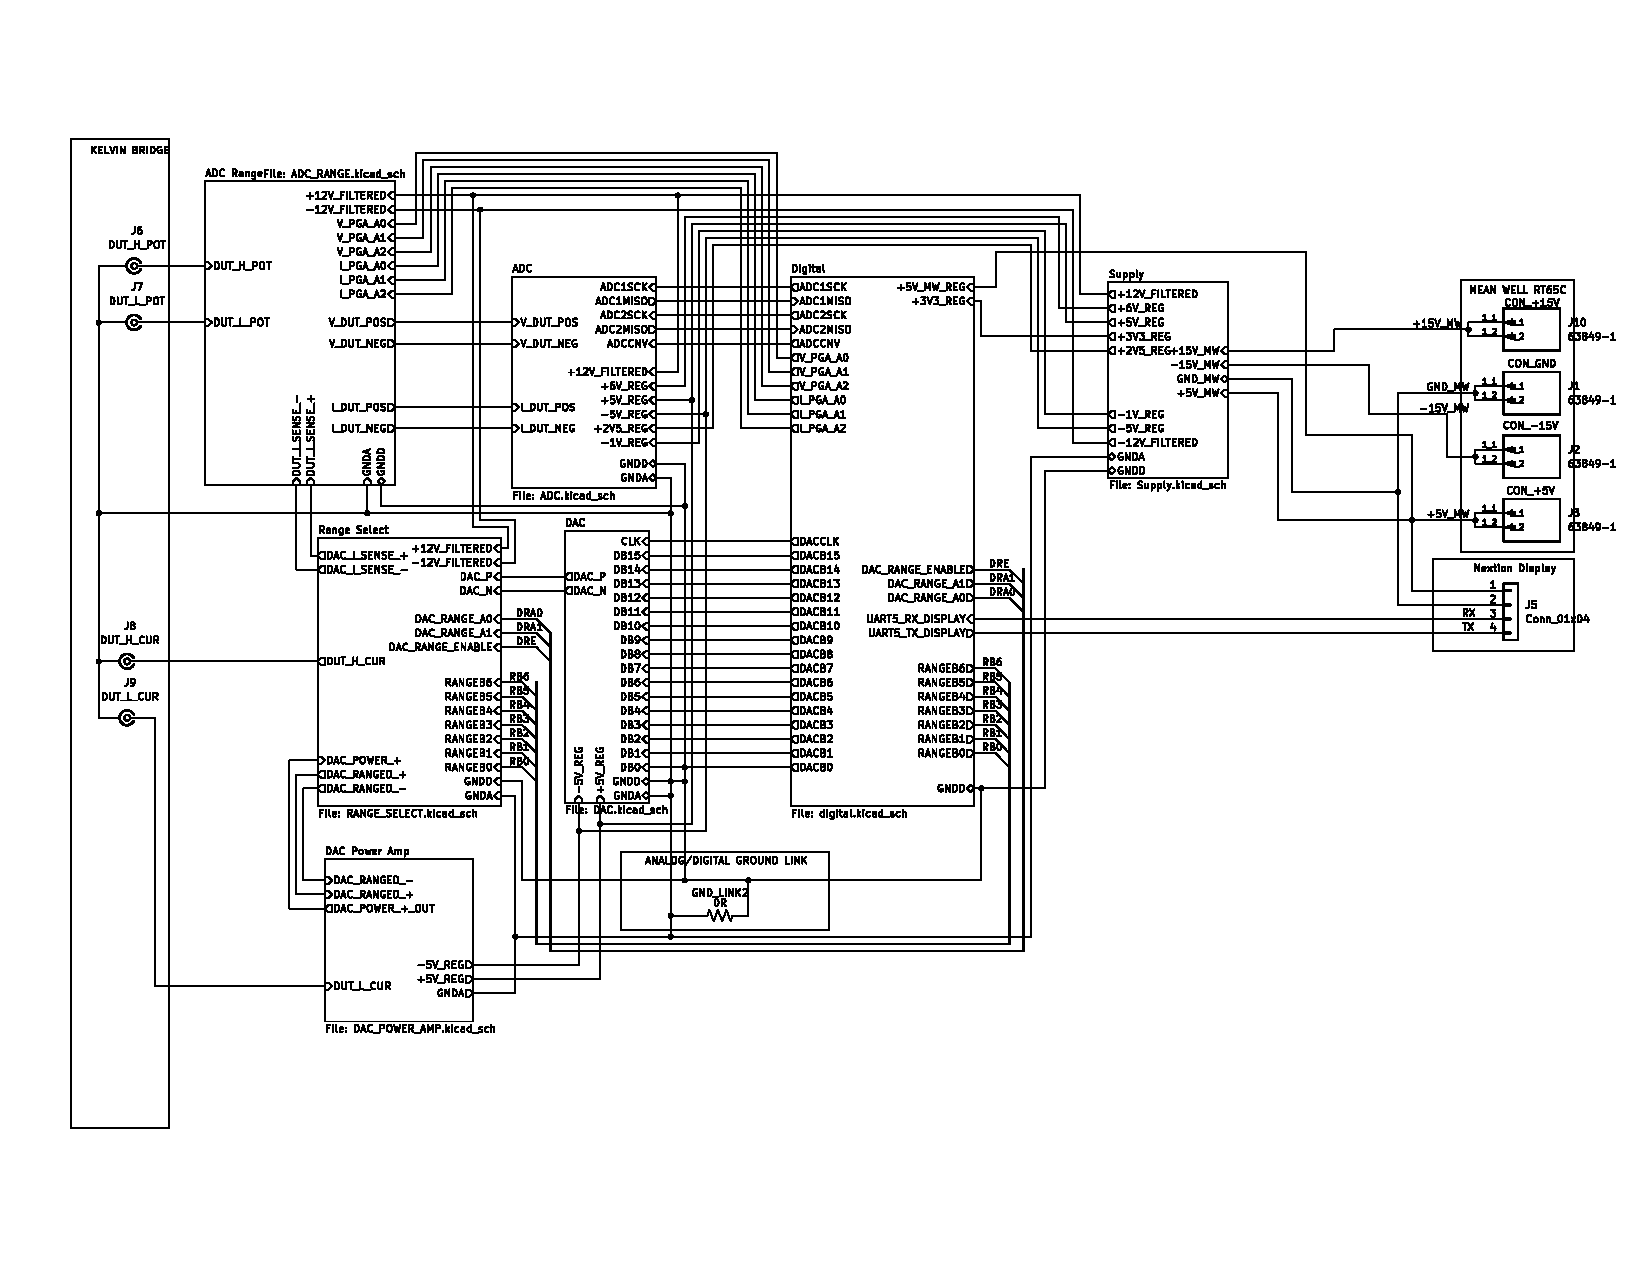
\includegraphics[clip, trim=0 50 0 0, width=1\textwidth]{Appendix/Figures/A_SCHEMATIC_TOPBLOCKS.pdf}
    \caption{The top layer of the schematic.}
    \label{fig_A_SCH_TOP}
\end{figure}

The ADC circuits, anti aliasing filters, ADC reference and offset circuits can be seen on figure \refq{fig_A_SCH_ADC}.

\begin{figure}[H]
    \centering
    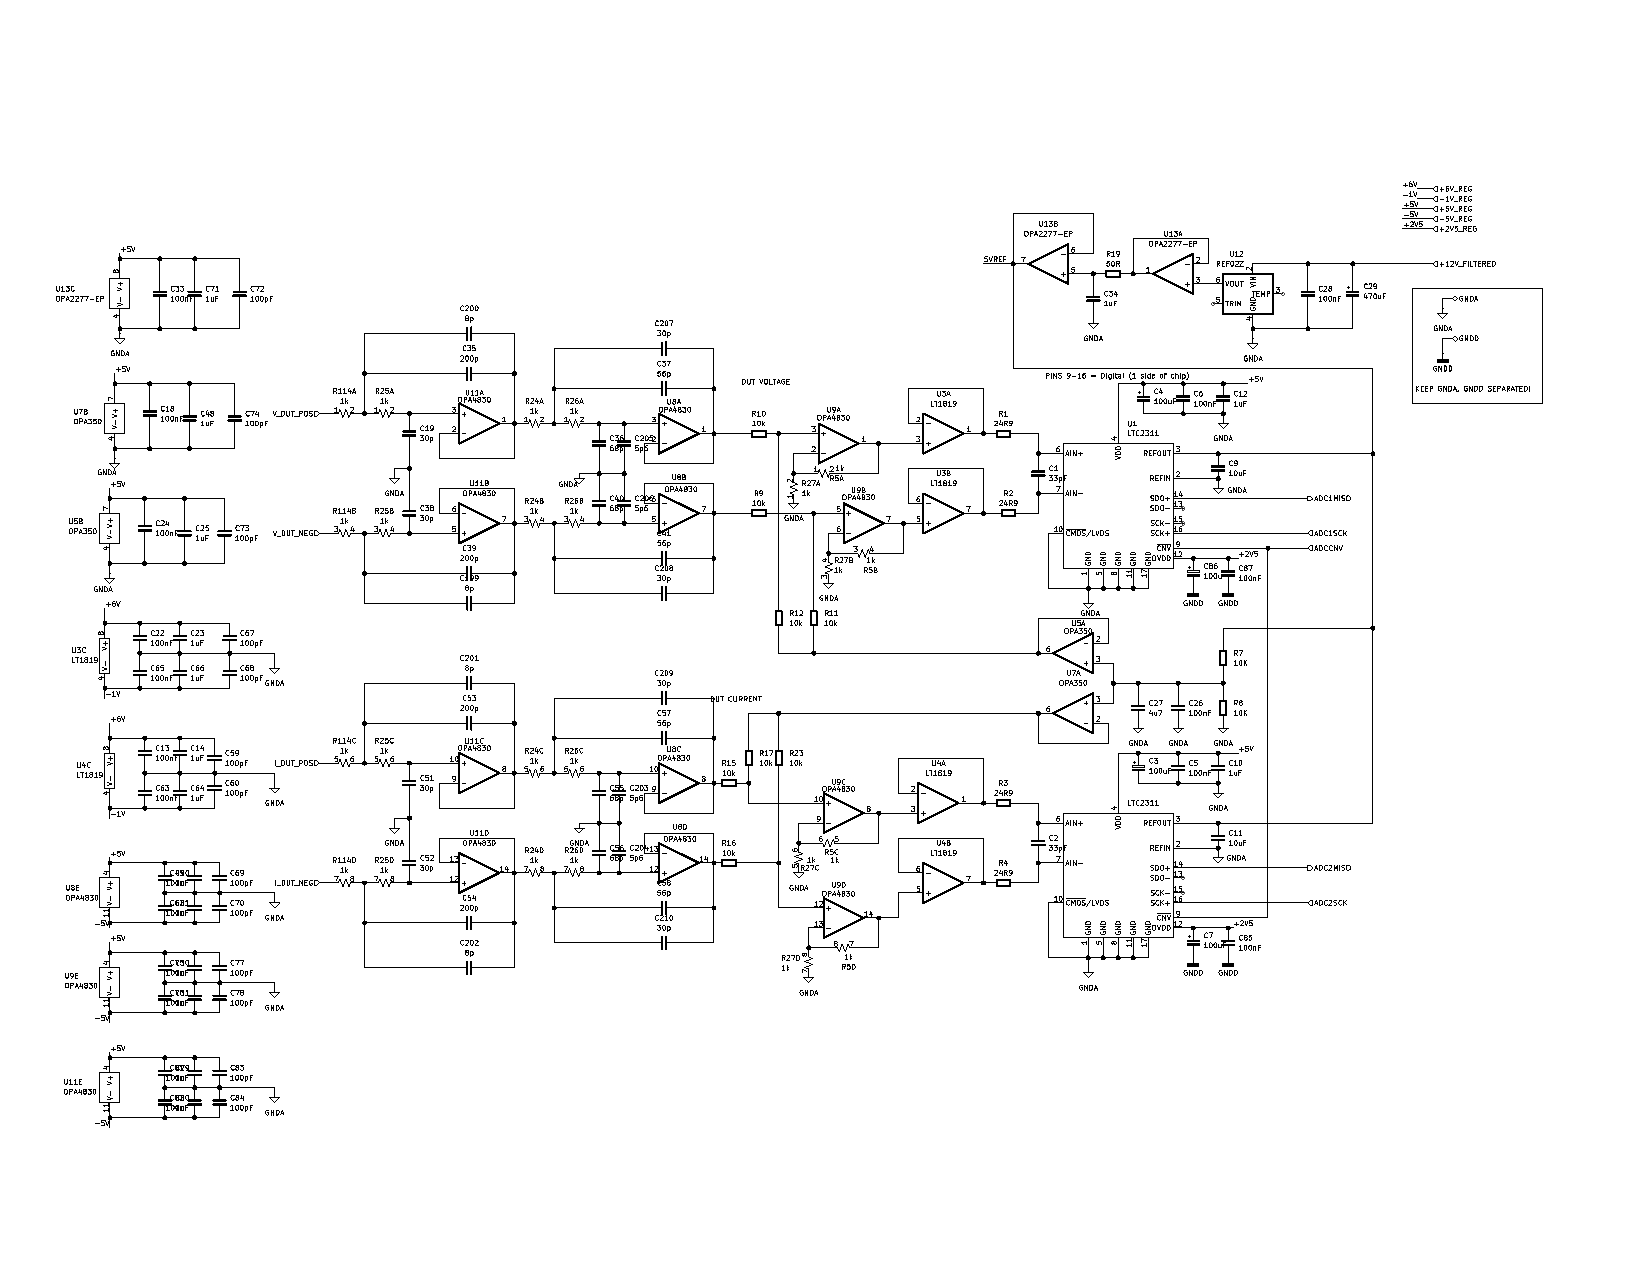
\includegraphics[clip, trim=0 50 0 0, width=1\textwidth]{Appendix/Figures/A_SCH_ADC.pdf}
    \caption{The schematic for the ADCs and supporting circuits.}
    \label{fig_A_SCH_ADC}
\end{figure}

The schematic for the DC supplies can be seen on figure \refq{fig_A_SCH_DCSUPPLY}.

\begin{figure}[H]
    \centering
    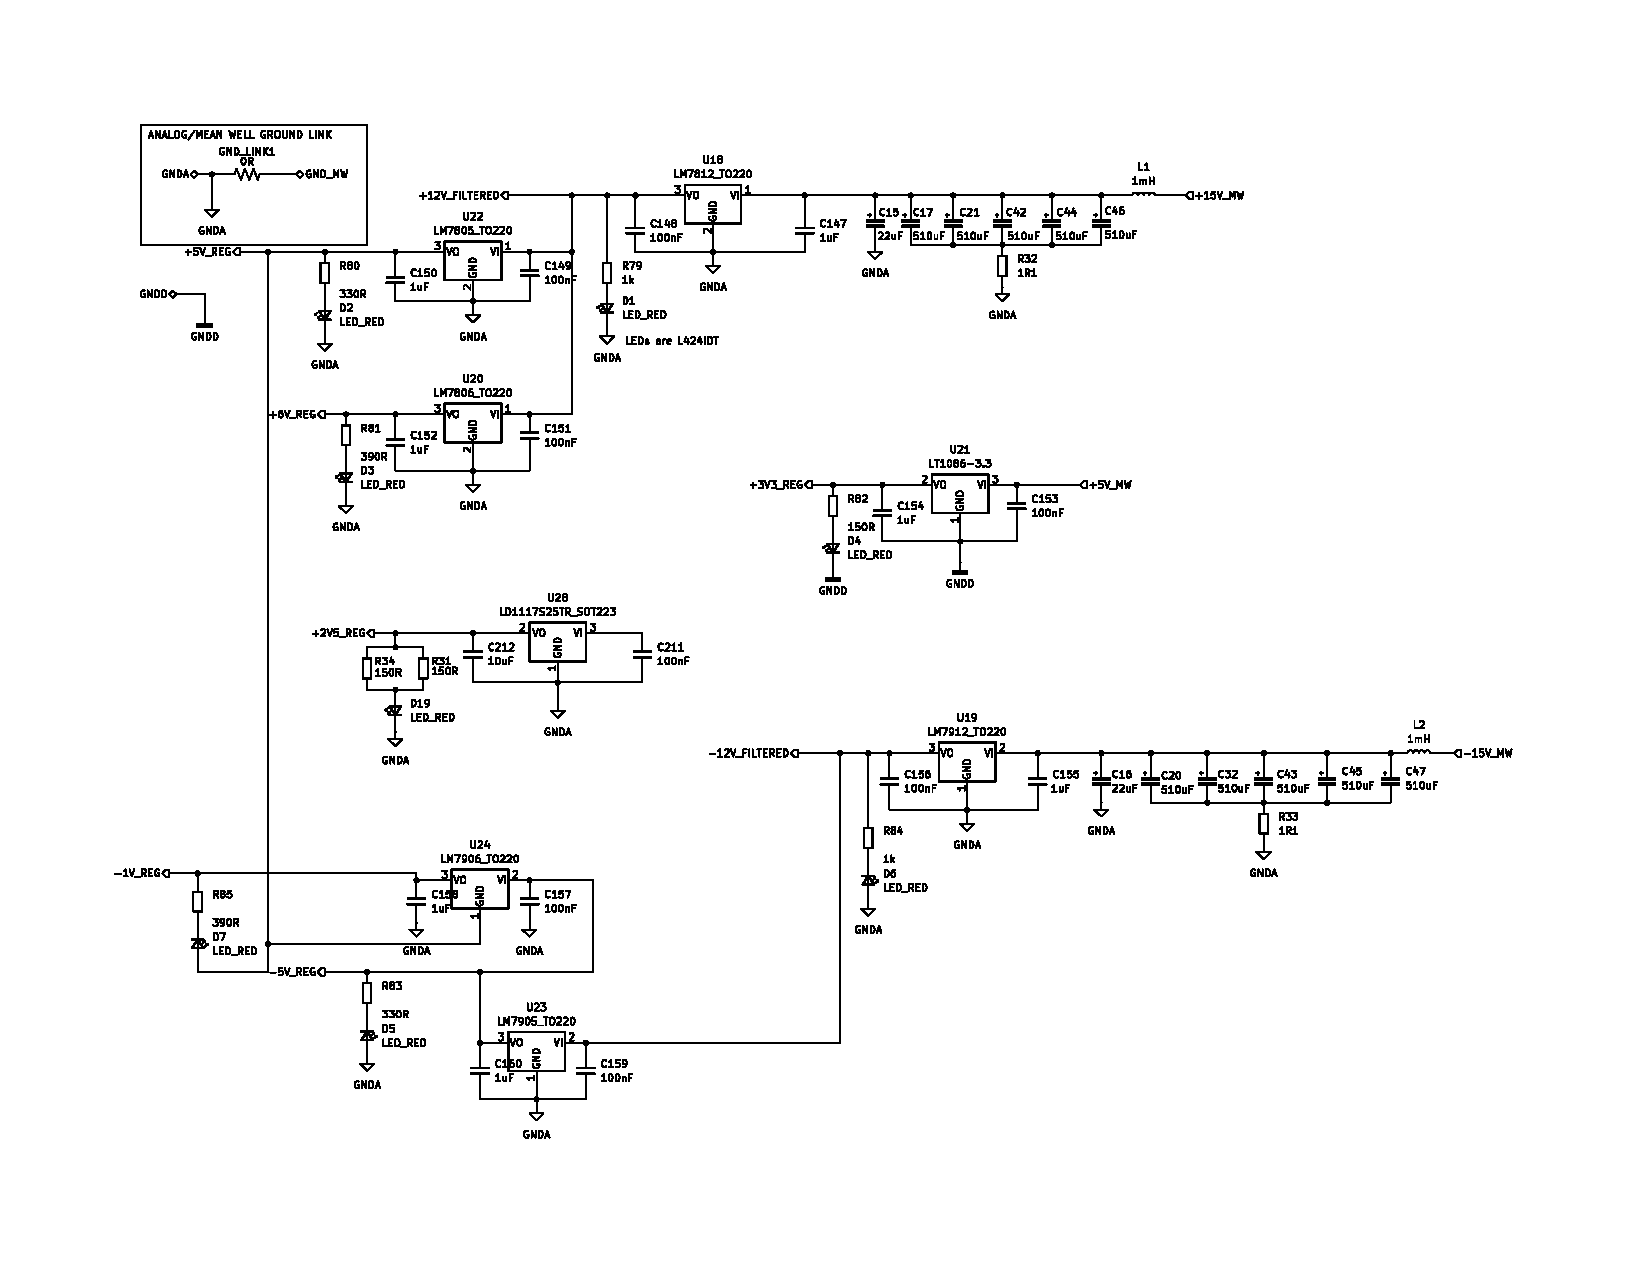
\includegraphics[clip, trim=0 50 0 0, width=1\textwidth]{Appendix/Figures/A_SCH_DCSUPPLY.pdf}
    \caption{The schematic for the DC supplies. The Mean Well RT65C external power supply is not shown on this schematic.}
    \label{fig_A_SCH_DCSUPPLY}
\end{figure}

The schematic for the DAC circuit and reconstruction filter can be seen on figure \refq{fig_A_SCH_DAC}.
\begin{figure}[H]
    \centering
    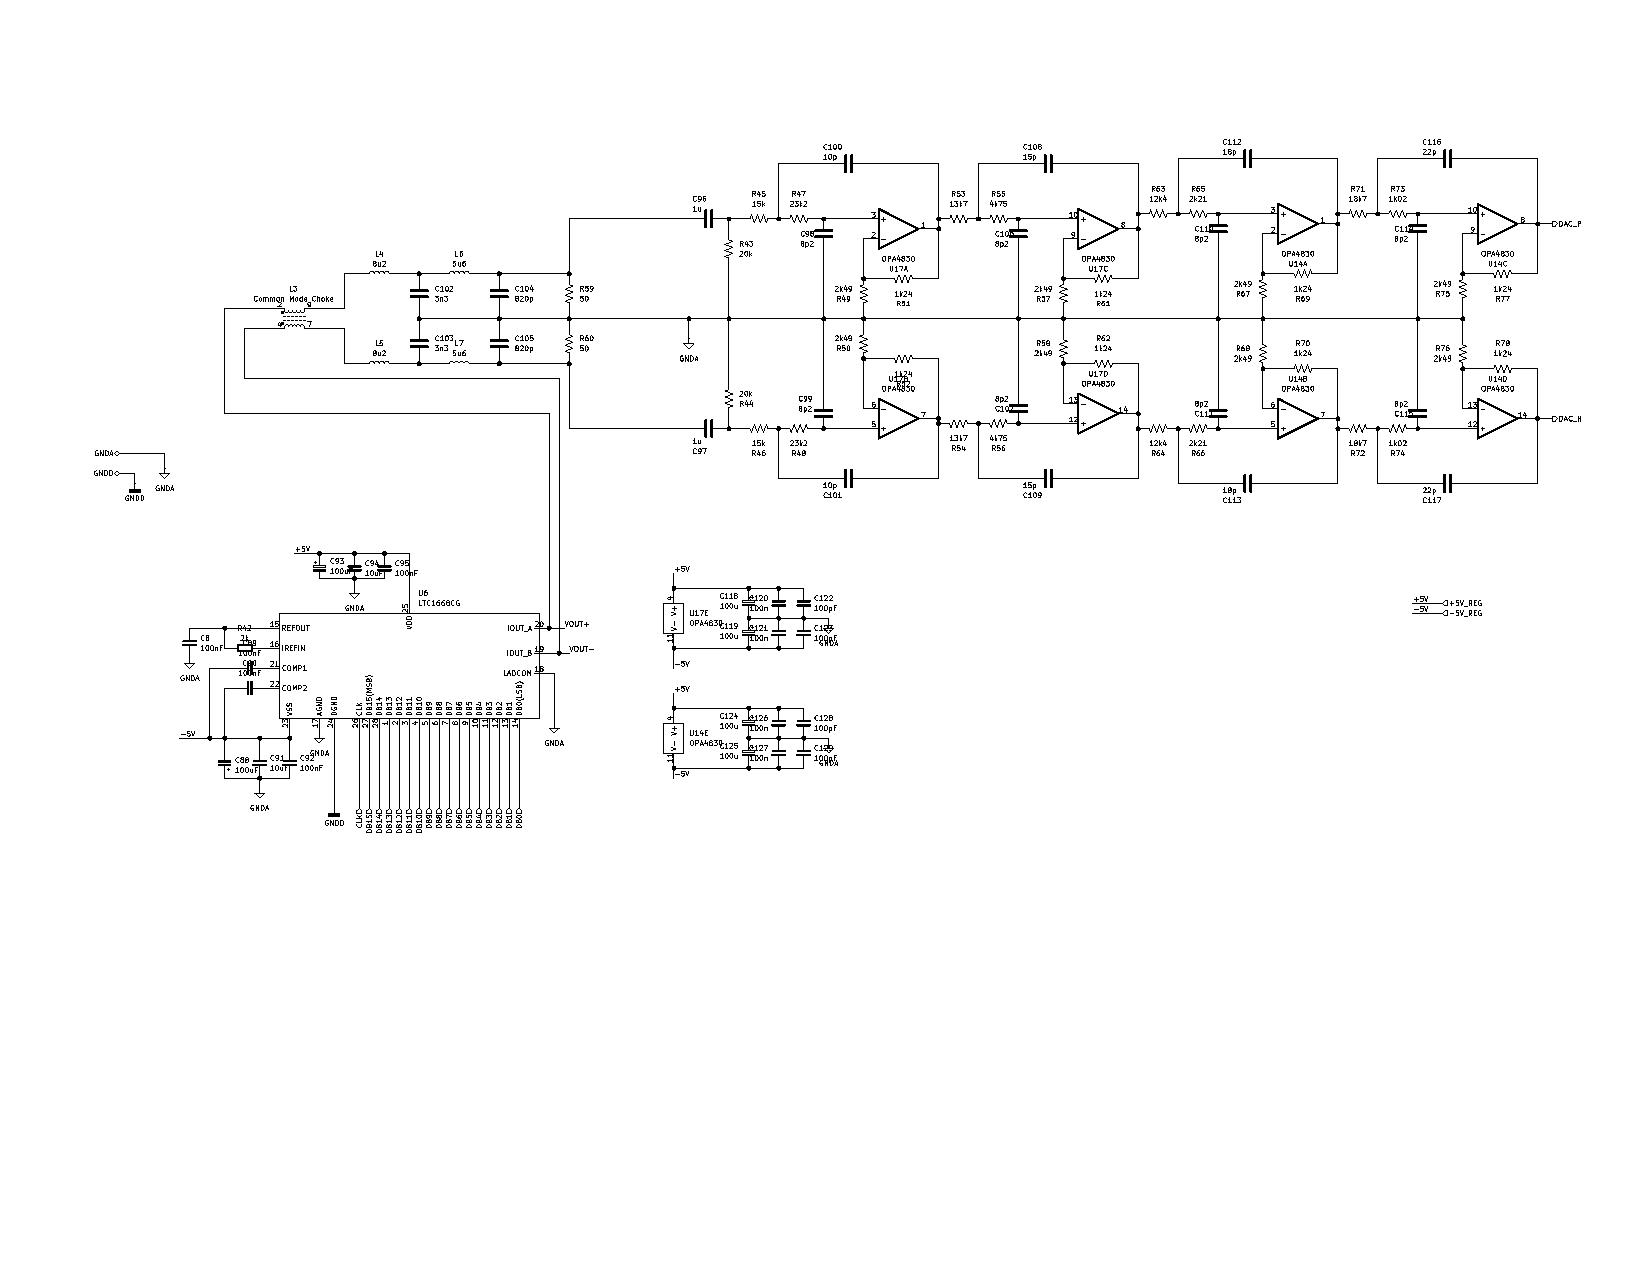
\includegraphics[clip, trim=0 200 0 0, width=1\textwidth]{Appendix/Figures/A_SCH_DAC.pdf}
    \caption{The schematic for the DAC and reconstruction filter.}
    \label{fig_A_SCH_DAC}
\end{figure}

The schematic for the digital circuits can be seen on figure \refq{fig_A_SCH_DIGITAL}.

\begin{figure}[H]
    \centering
    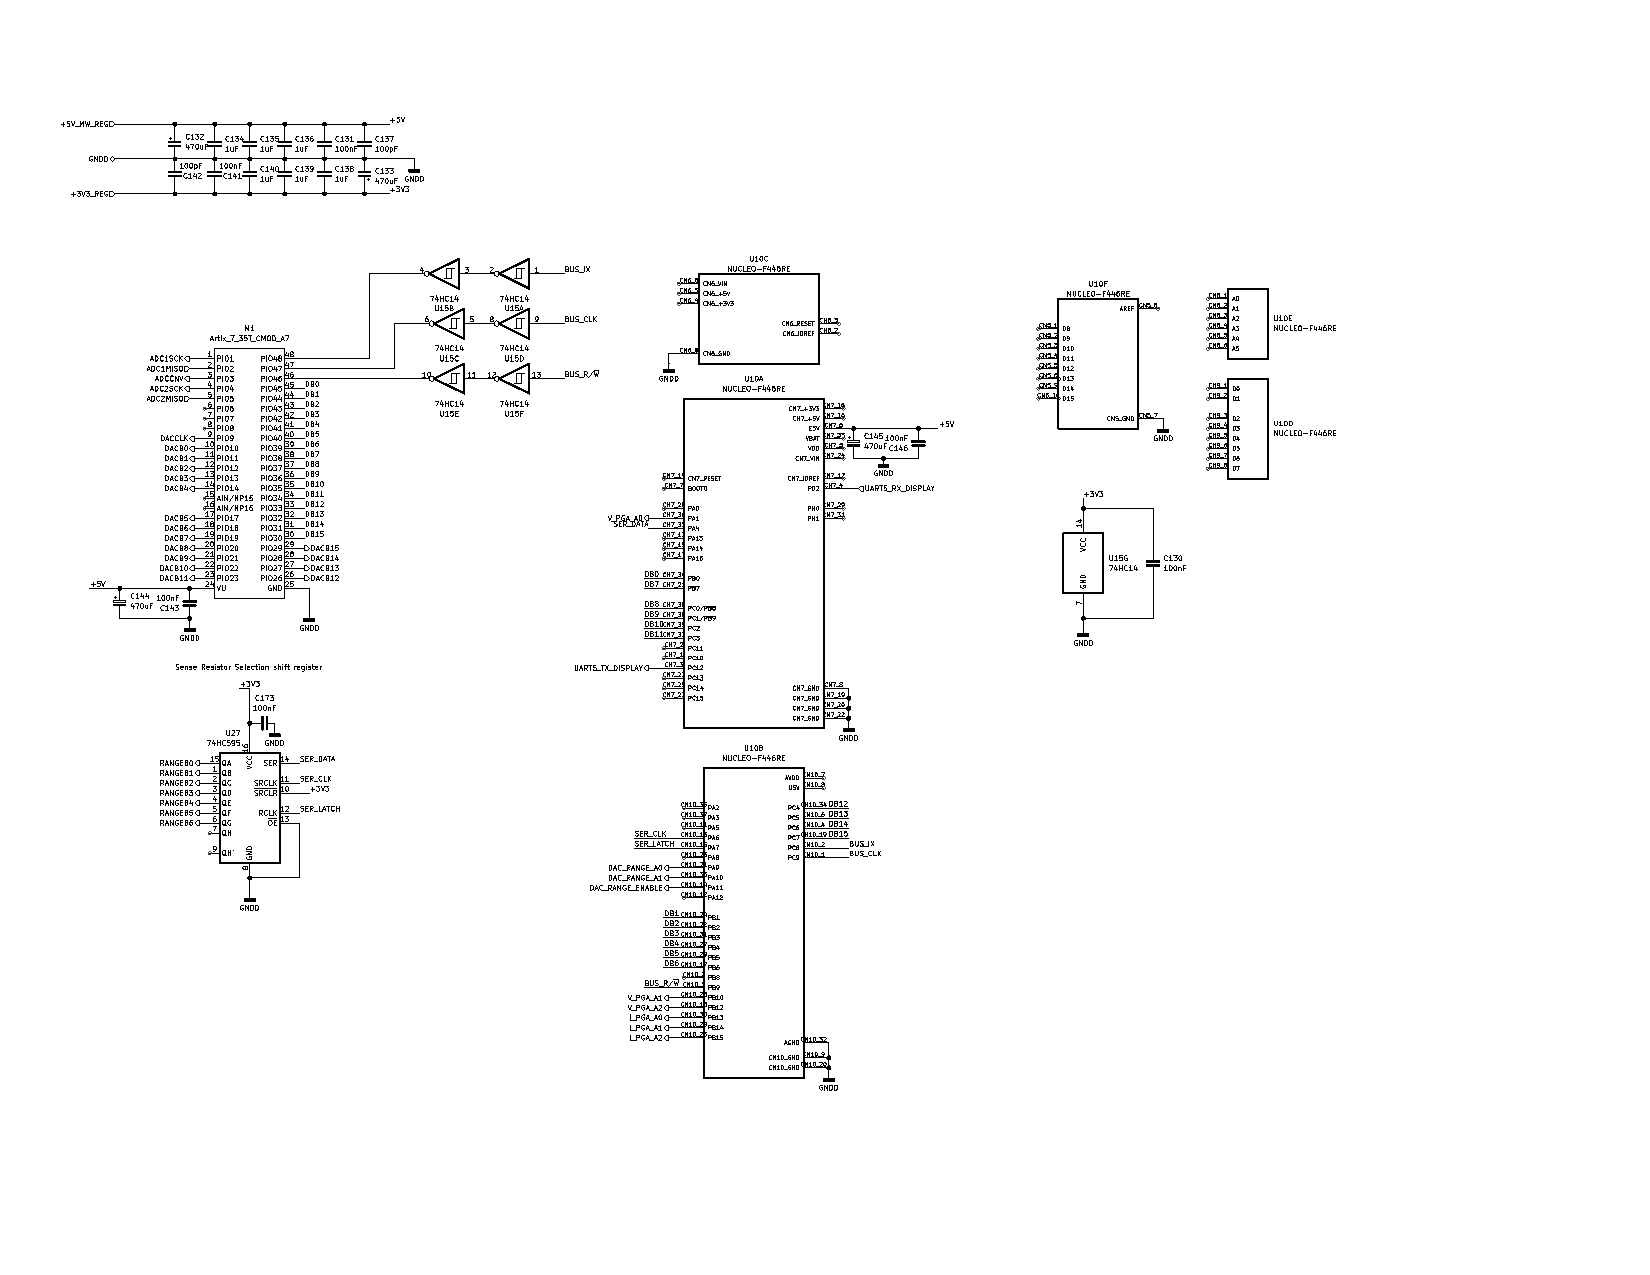
\includegraphics[clip, trim=0 50 0 0, width=1\textwidth]{Appendix/Figures/A_SCH_DIGITAL.pdf}
    \caption{The schematic for the digital circuits.}
    \label{fig_A_SCH_DIGITAL}
\end{figure}

The schematic for the programmable gain amplifiers can be seen on figure \refq{fig_A_SCH_PGA}.
\begin{figure}[H]
    \centering
    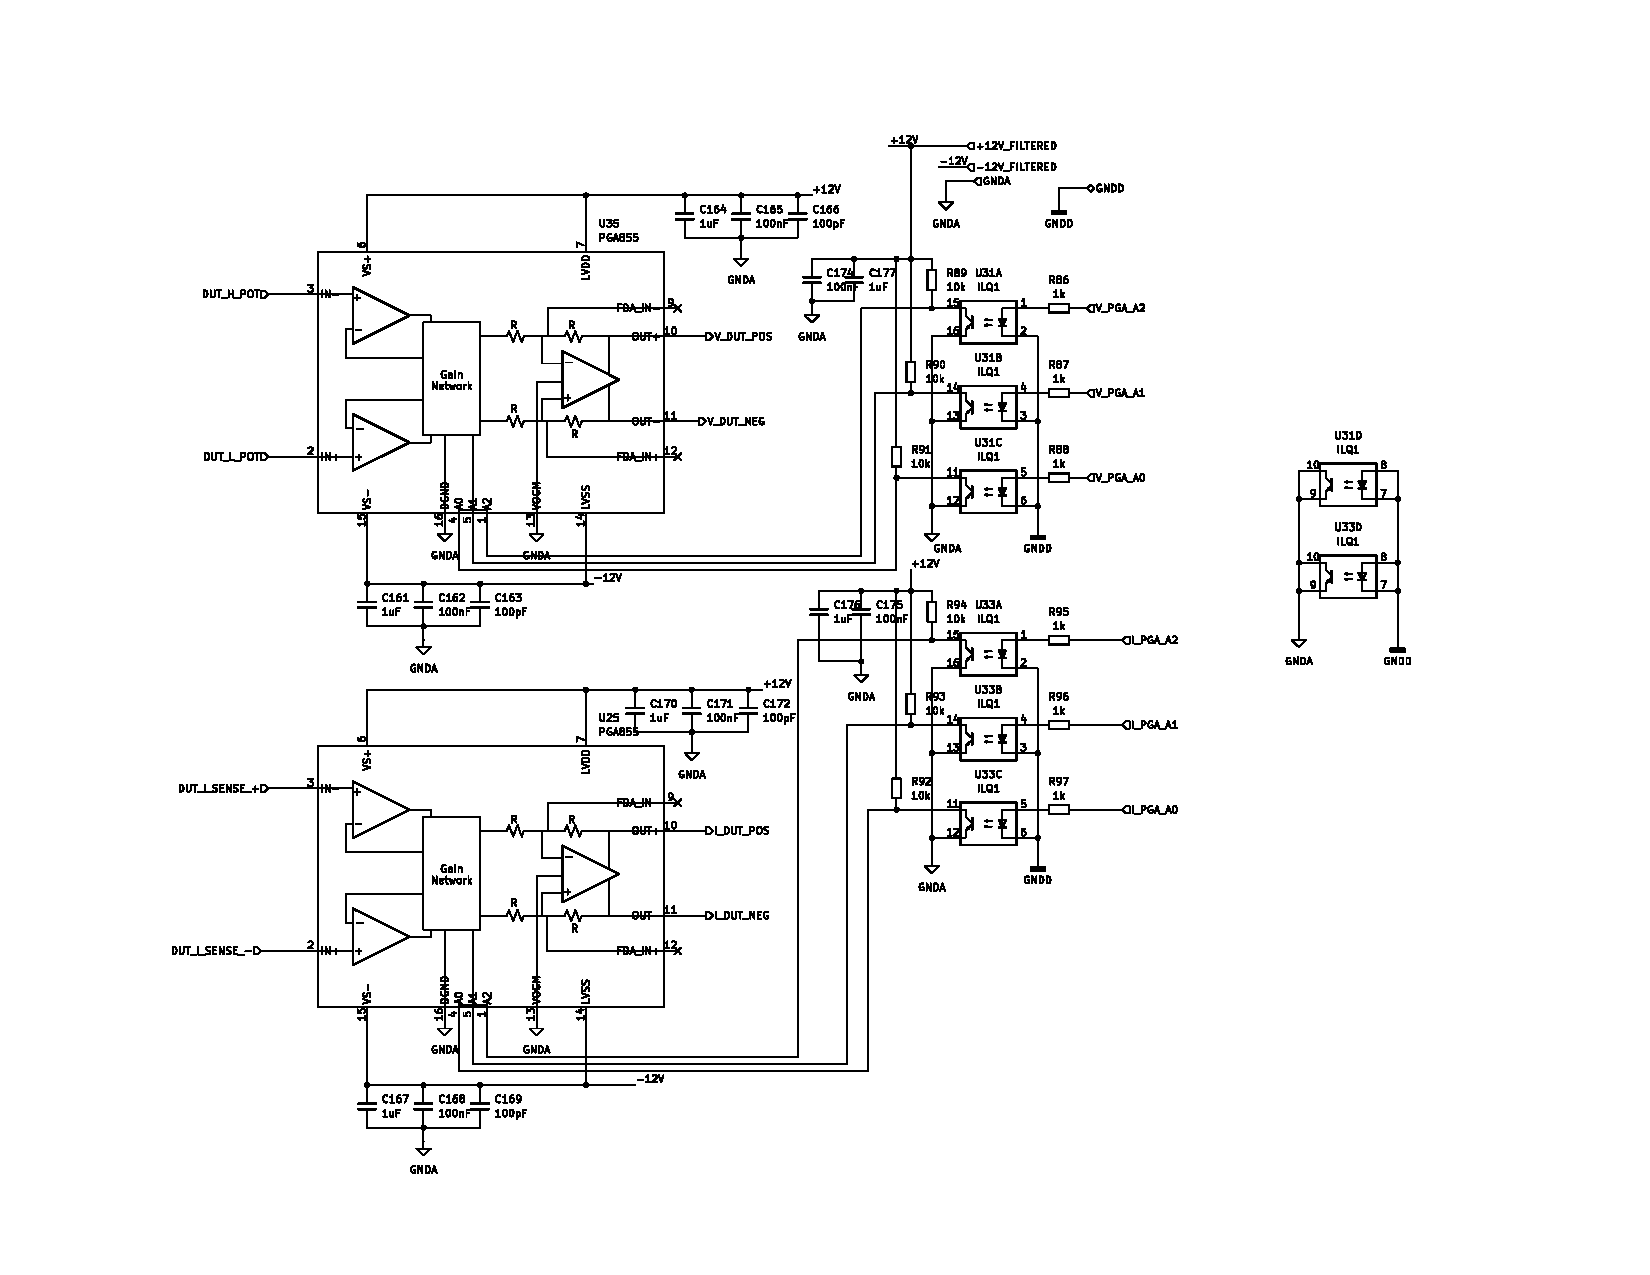
\includegraphics[clip, trim=0 25 0 0, width=1\textwidth]{Appendix/Figures/A_SCH_PGA.pdf}
    \caption{The schematic for the PGAs.}
    \label{fig_A_SCH_PGA}
\end{figure}

The schematic for the range selection circuit can be seen on figure \refq{fig_A_SCH_RANGE}.

\begin{figure}[H]
    \centering
    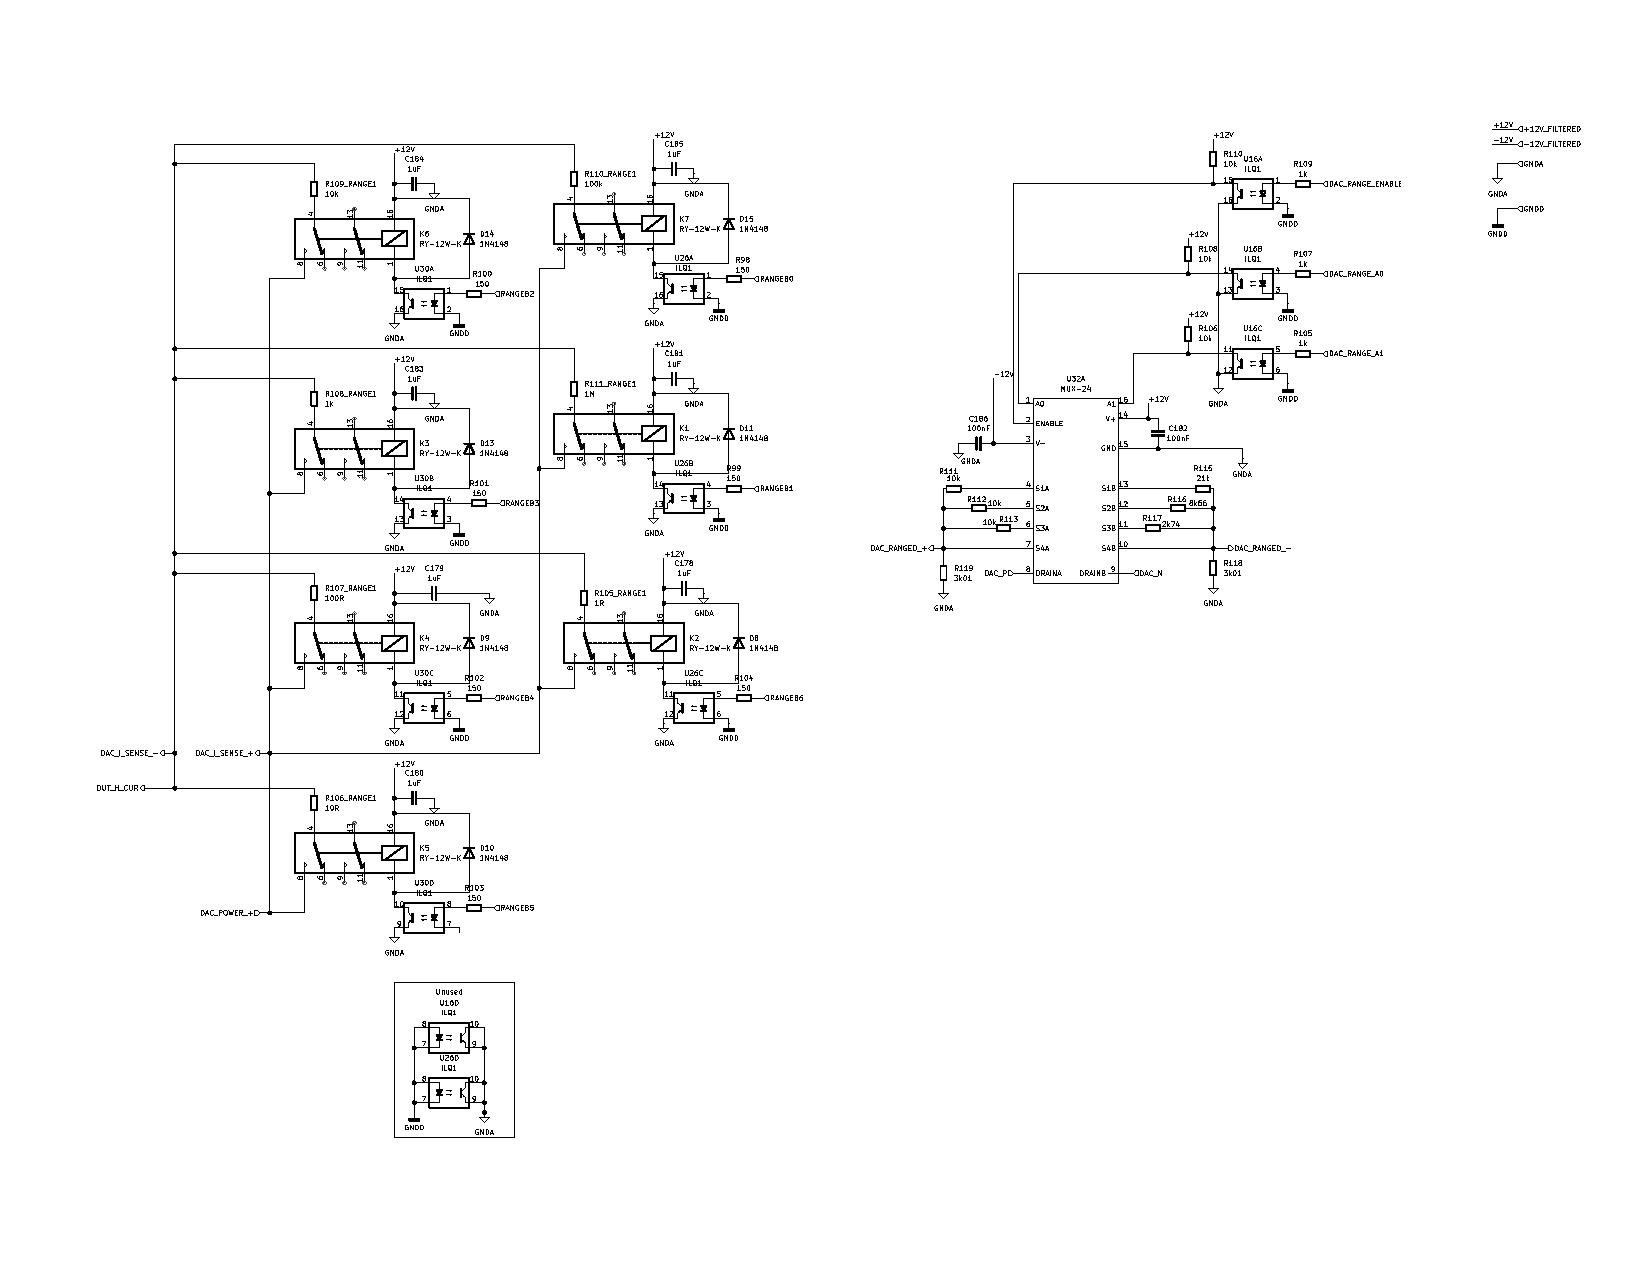
\includegraphics[clip, trim=0 25 0 0, width=1\textwidth]{Appendix/Figures/A_SCH_RANGE}
    \caption{The schematic for the range selection circuit.}
    \label{fig_A_SCH_RANGE}
\end{figure}

The schematic for the DAC power amplifier can be seen on figure \refq{fig_A_SCH_DACPA}
\begin{figure}[H]
    \centering
    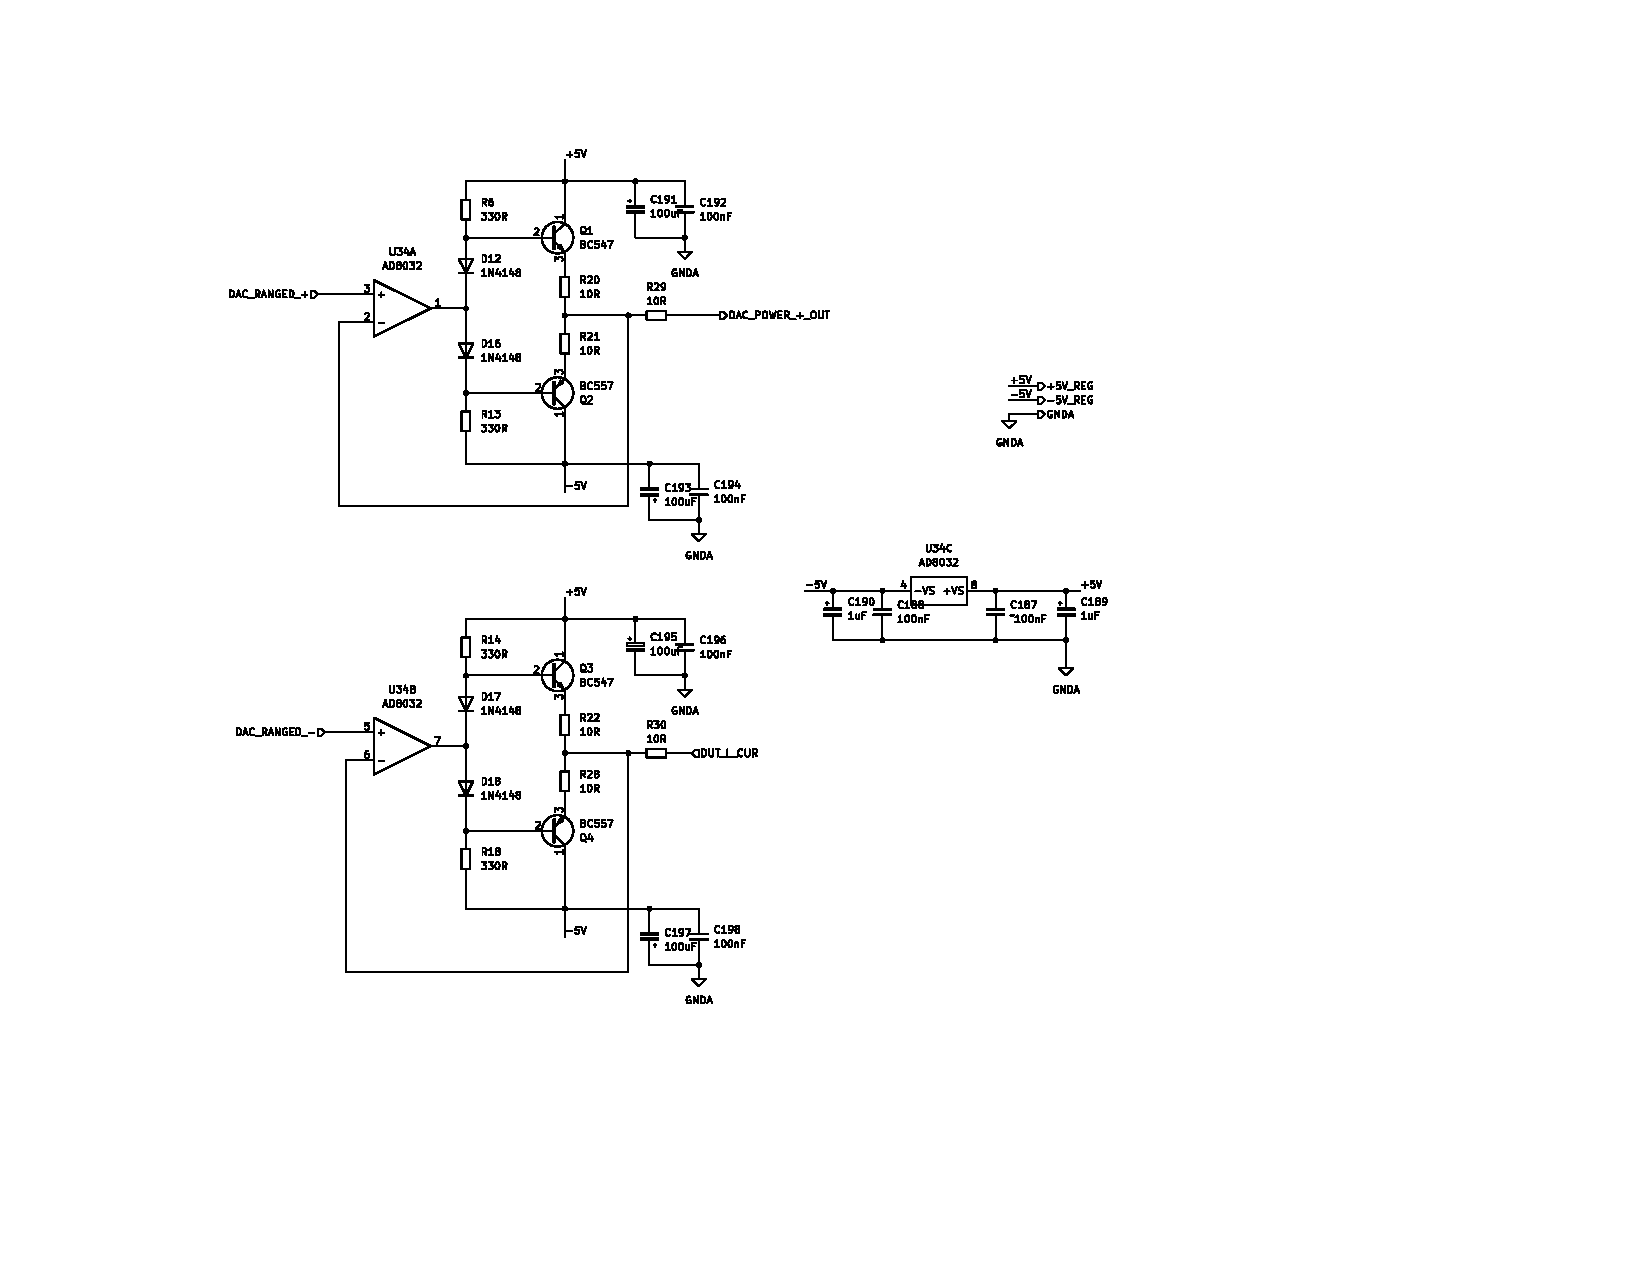
\includegraphics[clip, trim=0 100 0 0, width=1\textwidth]{Appendix/Figures/A_SCH_DACPA}
    \caption{The power amplifier circuit for the DAC.}
    \label{fig_A_SCH_DACPA}
\end{figure}